\subsection{Segmenta��o de Imagens \label{segmentacao_de_imagens}}

Em vis�o computacional, segmenta��o � o processo de dividir uma
imagem em m�ltiplas regi�es, com a inten��o de subdividir a imagem
em areas de interesse, ou simplesmente modific�-las, ambos a fim de
facilitar uma an�lise posterior. Em imagens monocrom�ticas
algoritmos de segmenta�ao s�o baseados em uma das propriedades b�sicas
de valores de n�veis de cinza: descontinuidade (detec��o de bordas) e
similaridade (agrupamento de regi�es homog�neas).

Na descontinuidade, o objetivo � particionar a imagem tendo como
regra mudan�as bruscas nas escalas de cinza. A similaridade
baseia-se na limiariza��o. A limiariza��o ou binariza��o de uma
imagem � dada a partir do n�vel de cinza de seus pixels. Tal
processo � dado pela defini��o de um limiar $T$ no histograma da imagem
e compara��o dos n�vel de tom de cinza dos pixels com o limiar $T$.
Valores que forem menores que a limiar, t�m seus valores de n�veis
de cinza aproximados para $255$, tornando-se brancos, e aqueles que
tiverem n�veis de cinza maiores que a limiar, t�m seus valores em
n�veis de cinza aproximados para 0, tornando-se pretos.

� dado um exemplo de histograma com limiar na Figura
\ref{img_seg_histograma}:

\begin{figure}[h|top]
 \centering
 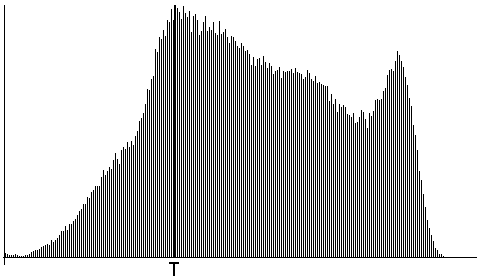
\includegraphics[width=1\linewidth]{imagens/seg_histograma.png}
 \caption{Exemplo de limiar com histograma.}
 \label{img_seg_histograma}
\end{figure}

\begin{figure}[ht]
	\begin{minipage}[b]{0.5\linewidth}
		\centering
		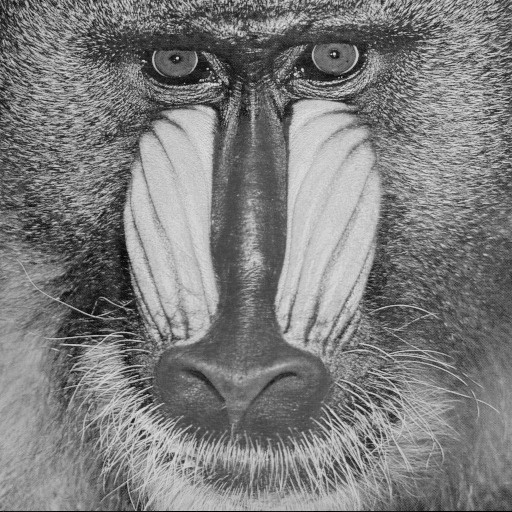
\includegraphics[scale=0.45]{imagens/seg_limiar_original.png}
		\caption{Imagem Original}
		\label{img:seg_limiar_original}
	\end{minipage}
	\hspace{0.5cm}
	\begin{minipage}[b]{0.5\linewidth}
		\centering
		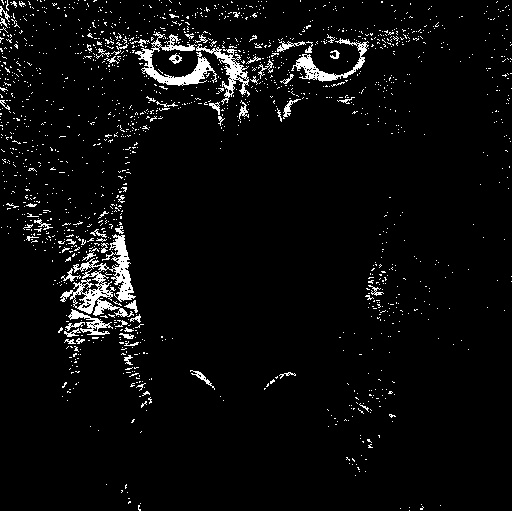
\includegraphics[scale=0.45]{imagens/seg_limiar_50.png}
		\caption{Limiar 50}
		\label{img:seg_limiar_50}
	\end{minipage}
\end{figure}

\begin{figure}[ht]
	\begin{minipage}[b]{0.5\linewidth}
		\centering
		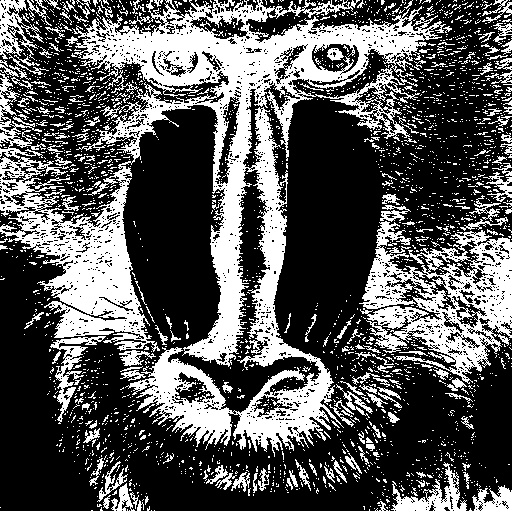
\includegraphics[scale=0.45]{imagens/seg_limiar_100.png}
		\caption{Limiar 100}
		\label{img:seg_limiar_100}
	\end{minipage}
	\hspace{0.5cm}
	\begin{minipage}[b]{0.5\linewidth}
		\centering
		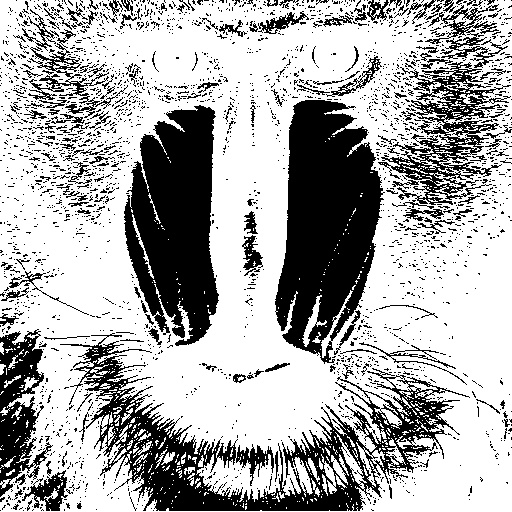
\includegraphics[scale=0.45]{imagens/seg_limiar_150.png}
		\caption{Limiar 150}
		\label{img:seg_limiar_150}
	\end{minipage}
\end{figure}

Como pode ser observado nos exemplos das Figuras \ref{img:seg_limiar_50},
\ref{img:seg_limiar_100} e \ref{img:seg_limiar_150}
dependendo do limiar escolhido o resultado se altera. Quanto menor o
valor da limiar mais pixels ter�o seus n�veis de cinza aproximados
de 255, deixando a imagem com mais pontos brancos do que pretos.
A rec�proca tambem e verdadeira. 
